\subsubsection{Exercise}

The two previous exercises lead to the design of the following controller:

$$F_r(s) = \frac{1}{1 + \tau s}$$
$$F_y(s) = K \frac{\tau_D s + 1}{\beta \tau_D s +1}\frac{s + \omega_I}{s} \frac{\omega_0^2}{(s+\omega_0)^2}G(s)^{-1} G_d(s)$$

With:

$$\begin{array}{rcl}
    \tau & = & 0.14 \text{ s}\\ 
    K &  = & 1.35\\
    \tau_D &  = & 0.078\text{ s}\\
    \beta &  = & 0.75\\
 \omega_I &  = & 5 \text{ rad.s}^{-1}\\
    \omega_0 &  = & 50 \text{ rad.s}^{-1}\\
\end{array}$$

\textbf{All the criteria are met:}

\begin{shortitemize}
    \item Rise time:
        $$t_r \leq 0.20\text{s}$$
    \item Overshoot:
        $$D(\%) \leq 10\%$$
    \item Step in the disturbance:
        $$|y(t)| \leq 1, \forall t \text{ and } |y(t)| \leq 0.1, \forall t \geq 0.5\text{ s}$$ 
    \item Control signal obeys:
        $$|u(t)| \leq 1, \forall t$$
\end{shortitemize}

Figure \ref{designFr} shows the step response of the system, the response to a step in the disturbance and the bode diagram of the sensitivity and complementary sensitivity functions.

\begin{figure}[h!t]
    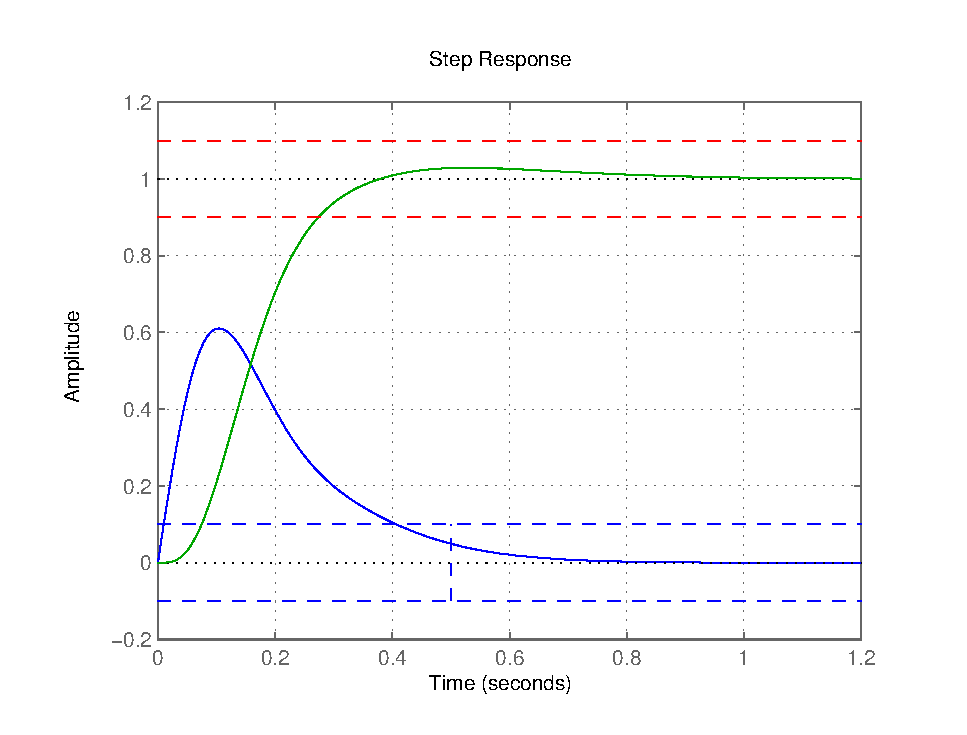
\includegraphics[width=\columnwidth]{fig/designFr.eps}
    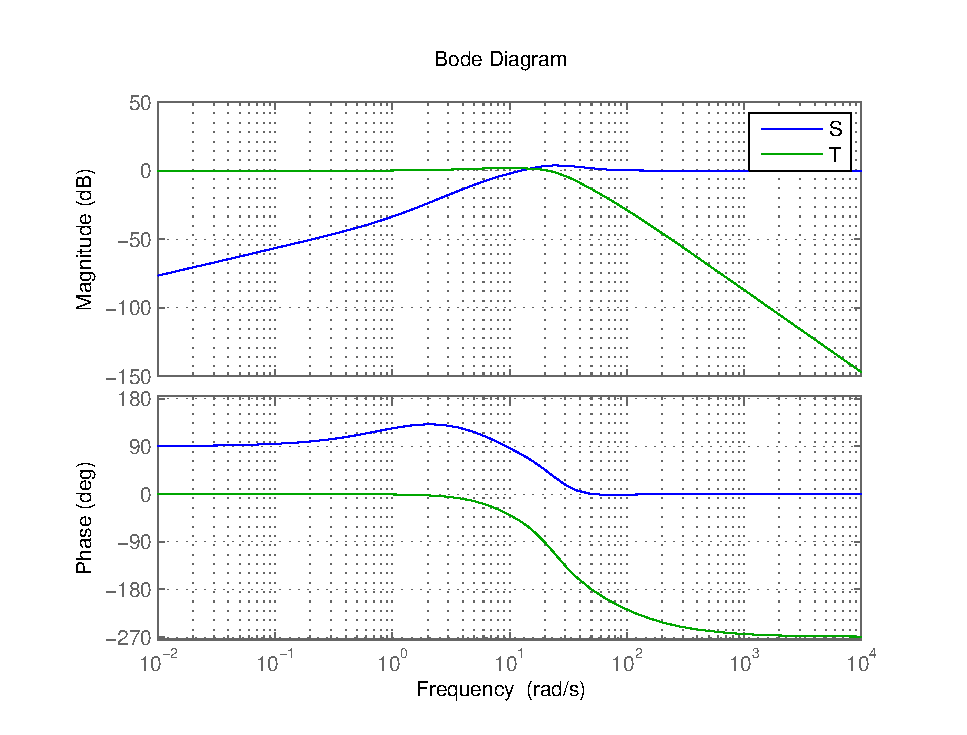
\includegraphics[width=\columnwidth]{fig/sensitivitiesFunction.eps}
    \caption{Step response of the system (green) and response to a step in the disturbance (blue) with the addition of the lead-controller \\ Bode diagram of the sensitivity and complementary sensitivity functions}
    \label{designFr}
\end{figure}

